% Options for packages loaded elsewhere
\PassOptionsToPackage{unicode}{hyperref}
\PassOptionsToPackage{hyphens}{url}
%
\documentclass[
]{article}
\usepackage{amsmath,amssymb}
\usepackage{lmodern}
\usepackage{ifxetex,ifluatex}
\ifnum 0\ifxetex 1\fi\ifluatex 1\fi=0 % if pdftex
  \usepackage[T1]{fontenc}
  \usepackage[utf8]{inputenc}
  \usepackage{textcomp} % provide euro and other symbols
\else % if luatex or xetex
  \usepackage{unicode-math}
  \defaultfontfeatures{Scale=MatchLowercase}
  \defaultfontfeatures[\rmfamily]{Ligatures=TeX,Scale=1}
\fi
% Use upquote if available, for straight quotes in verbatim environments
\IfFileExists{upquote.sty}{\usepackage{upquote}}{}
\IfFileExists{microtype.sty}{% use microtype if available
  \usepackage[]{microtype}
  \UseMicrotypeSet[protrusion]{basicmath} % disable protrusion for tt fonts
}{}
\makeatletter
\@ifundefined{KOMAClassName}{% if non-KOMA class
  \IfFileExists{parskip.sty}{%
    \usepackage{parskip}
  }{% else
    \setlength{\parindent}{0pt}
    \setlength{\parskip}{6pt plus 2pt minus 1pt}}
}{% if KOMA class
  \KOMAoptions{parskip=half}}
\makeatother
\usepackage{xcolor}
\IfFileExists{xurl.sty}{\usepackage{xurl}}{} % add URL line breaks if available
\IfFileExists{bookmark.sty}{\usepackage{bookmark}}{\usepackage{hyperref}}
\hypersetup{
  pdftitle={Informe-ElPrecioDeLaDiscapacidad},
  hidelinks,
  pdfcreator={LaTeX via pandoc}}
\urlstyle{same} % disable monospaced font for URLs
\usepackage[margin=1in]{geometry}
\usepackage{color}
\usepackage{fancyvrb}
\newcommand{\VerbBar}{|}
\newcommand{\VERB}{\Verb[commandchars=\\\{\}]}
\DefineVerbatimEnvironment{Highlighting}{Verbatim}{commandchars=\\\{\}}
% Add ',fontsize=\small' for more characters per line
\usepackage{framed}
\definecolor{shadecolor}{RGB}{248,248,248}
\newenvironment{Shaded}{\begin{snugshade}}{\end{snugshade}}
\newcommand{\AlertTok}[1]{\textcolor[rgb]{0.94,0.16,0.16}{#1}}
\newcommand{\AnnotationTok}[1]{\textcolor[rgb]{0.56,0.35,0.01}{\textbf{\textit{#1}}}}
\newcommand{\AttributeTok}[1]{\textcolor[rgb]{0.77,0.63,0.00}{#1}}
\newcommand{\BaseNTok}[1]{\textcolor[rgb]{0.00,0.00,0.81}{#1}}
\newcommand{\BuiltInTok}[1]{#1}
\newcommand{\CharTok}[1]{\textcolor[rgb]{0.31,0.60,0.02}{#1}}
\newcommand{\CommentTok}[1]{\textcolor[rgb]{0.56,0.35,0.01}{\textit{#1}}}
\newcommand{\CommentVarTok}[1]{\textcolor[rgb]{0.56,0.35,0.01}{\textbf{\textit{#1}}}}
\newcommand{\ConstantTok}[1]{\textcolor[rgb]{0.00,0.00,0.00}{#1}}
\newcommand{\ControlFlowTok}[1]{\textcolor[rgb]{0.13,0.29,0.53}{\textbf{#1}}}
\newcommand{\DataTypeTok}[1]{\textcolor[rgb]{0.13,0.29,0.53}{#1}}
\newcommand{\DecValTok}[1]{\textcolor[rgb]{0.00,0.00,0.81}{#1}}
\newcommand{\DocumentationTok}[1]{\textcolor[rgb]{0.56,0.35,0.01}{\textbf{\textit{#1}}}}
\newcommand{\ErrorTok}[1]{\textcolor[rgb]{0.64,0.00,0.00}{\textbf{#1}}}
\newcommand{\ExtensionTok}[1]{#1}
\newcommand{\FloatTok}[1]{\textcolor[rgb]{0.00,0.00,0.81}{#1}}
\newcommand{\FunctionTok}[1]{\textcolor[rgb]{0.00,0.00,0.00}{#1}}
\newcommand{\ImportTok}[1]{#1}
\newcommand{\InformationTok}[1]{\textcolor[rgb]{0.56,0.35,0.01}{\textbf{\textit{#1}}}}
\newcommand{\KeywordTok}[1]{\textcolor[rgb]{0.13,0.29,0.53}{\textbf{#1}}}
\newcommand{\NormalTok}[1]{#1}
\newcommand{\OperatorTok}[1]{\textcolor[rgb]{0.81,0.36,0.00}{\textbf{#1}}}
\newcommand{\OtherTok}[1]{\textcolor[rgb]{0.56,0.35,0.01}{#1}}
\newcommand{\PreprocessorTok}[1]{\textcolor[rgb]{0.56,0.35,0.01}{\textit{#1}}}
\newcommand{\RegionMarkerTok}[1]{#1}
\newcommand{\SpecialCharTok}[1]{\textcolor[rgb]{0.00,0.00,0.00}{#1}}
\newcommand{\SpecialStringTok}[1]{\textcolor[rgb]{0.31,0.60,0.02}{#1}}
\newcommand{\StringTok}[1]{\textcolor[rgb]{0.31,0.60,0.02}{#1}}
\newcommand{\VariableTok}[1]{\textcolor[rgb]{0.00,0.00,0.00}{#1}}
\newcommand{\VerbatimStringTok}[1]{\textcolor[rgb]{0.31,0.60,0.02}{#1}}
\newcommand{\WarningTok}[1]{\textcolor[rgb]{0.56,0.35,0.01}{\textbf{\textit{#1}}}}
\usepackage{graphicx}
\makeatletter
\def\maxwidth{\ifdim\Gin@nat@width>\linewidth\linewidth\else\Gin@nat@width\fi}
\def\maxheight{\ifdim\Gin@nat@height>\textheight\textheight\else\Gin@nat@height\fi}
\makeatother
% Scale images if necessary, so that they will not overflow the page
% margins by default, and it is still possible to overwrite the defaults
% using explicit options in \includegraphics[width, height, ...]{}
\setkeys{Gin}{width=\maxwidth,height=\maxheight,keepaspectratio}
% Set default figure placement to htbp
\makeatletter
\def\fps@figure{htbp}
\makeatother
\setlength{\emergencystretch}{3em} % prevent overfull lines
\providecommand{\tightlist}{%
  \setlength{\itemsep}{0pt}\setlength{\parskip}{0pt}}
\setcounter{secnumdepth}{-\maxdimen} % remove section numbering
\ifluatex
  \usepackage{selnolig}  % disable illegal ligatures
\fi

\title{Informe-ElPrecioDeLaDiscapacidad}
\author{}
\date{\vspace{-2.5em}null}

\begin{document}
\maketitle

\hypertarget{informaciuxf3n-introductoria}{%
\subsubsection{Información
introductoria:}\label{informaciuxf3n-introductoria}}

\hypertarget{r-markdown}{%
\subsection{R Markdown}\label{r-markdown}}

This is an R Markdown document. Markdown is a simple formatting syntax
for authoring HTML, PDF, and MS Word documents. For more details on
using R Markdown see \url{http://rmarkdown.rstudio.com}.

When you click the \textbf{Knit} button a document will be generated
that includes both content as well as the output of any embedded R code
chunks within the document. You can embed an R code chunk like this:

\begin{Shaded}
\begin{Highlighting}[]
\FunctionTok{summary}\NormalTok{(cars)}
\end{Highlighting}
\end{Shaded}

\begin{verbatim}
##      speed           dist       
##  Min.   : 4.0   Min.   :  2.00  
##  1st Qu.:12.0   1st Qu.: 26.00  
##  Median :15.0   Median : 36.00  
##  Mean   :15.4   Mean   : 42.98  
##  3rd Qu.:19.0   3rd Qu.: 56.00  
##  Max.   :25.0   Max.   :120.00
\end{verbatim}

\hypertarget{including-plots}{%
\subsection{Including Plots}\label{including-plots}}

You can also embed plots, for example:

\includegraphics{Informe-ElPrecioDeLaDiscapacidad_files/figure-latex/pressure-1.pdf}

Note that the \texttt{echo\ =\ FALSE} parameter was added to the code
chunk to prevent printing of the R code that generated the plot.

\hypertarget{el-precio-de-la-discapacidad}{%
\section{EL PRECIO DE LA
DISCAPACIDAD}\label{el-precio-de-la-discapacidad}}

\hypertarget{introducciuxf3n}{%
\subsection{Introducción:}\label{introducciuxf3n}}

Las palabras textuales con las que la Real Academia Española (RAE)
define el término ``discapacidad'' son: \emph{``Situación de la persona
que por sus condiciones físicas o mentales duraderas se enfrenta con
notables barreras de acceso a su participación social''}. Sin embargo,
¿el \textbf{entorno} supone aún más barreras para las personas
discapacitadas? En este trabajo pretendemos responder a esta pregunta y
muchas otras relacionadas, porque sospechamos que el contexto que rodea
a un individuo discapacitado está íntimamente relacionado con la
aparición de dicha minusvalía y su posterior desarrollo.

En primer lugar, sabemos que está demostrado que el entorno en el que
vivimos afecta directamente en la manera cómo percibimos la sociedad y
cómo interactuamos con ella. Precisamente, nos interesa analizar este
último punto porque las personas con las que se relacione un individuo,
los alimentos que ingiera, o, simplemente, las acciones que lleve a cabo
pueden afectar a su salud; y, por tanto, ser \textbf{causa} de que
aparezca una discapacidad. Incluso, si nos adentramos aún más, las
características del lugar donde vive un sujeto, las cuales son
inamovibles, también pueden influir en la probabilidad de padecer una
minusvalía, por ejemplo, la contaminación.

Por otro lado, queremos comprobar hasta qué punto limita a un
discapacitado vivir en un \textbf{lugar} u otro. En concreto, vamos a
comparar las diferencias entre las facilidades que aporta el
\textbf{medio urbano} y el \textbf{medio rural}. Normalmente la
tranquilidad presente en los pueblos, por su cercanía con la naturaleza,
es algo satisfactorio para el estado psicológico de los minusválidos;
sin embargo, las ciudades presentan disponibles muchos más servicios
clínicos que ayudan a tratar la patología.

Finalmente, nos interesa conocer no sólo los datos estadísticos que den
respuesta a nuestras cuestiones, sino también las opiniones de
individuos discapacitados que hayan padecido en sus propias carnes estos
dilemas y puedan ser realistas exponiendo cómo se sienten. Así podremos
analizar los \textbf{cambios sociales y administrativos} que se
necesitan en este ámbito dando voz a este sector en ocasiones ignorado.

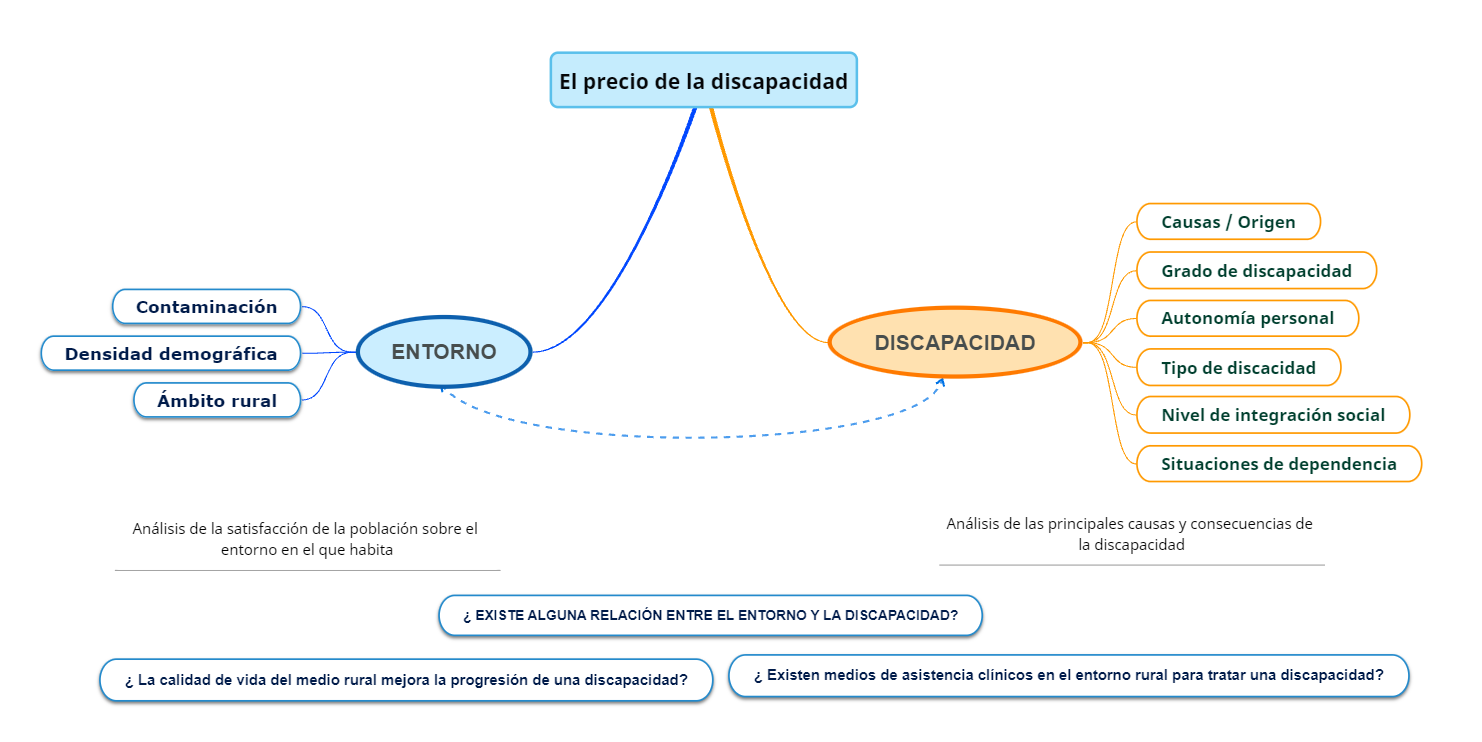
\includegraphics{C:/Users/usuario/Documents/INGENIERIA DE LA SALUD/3º UNI GIS/FUENTES DE DATOS BIOMÉDICAS Y WEB SEMÁNTICAS/El precio de la discapacidad/infoObjetivosSeminario.png}

\hypertarget{objetivos}{%
\subsection{Objetivos:}\label{objetivos}}

Teniendo en cuenta las secciones que trataremos, previamente descritas
en la introducción, vamos a enumerar los objetivos del trabajo.

\begin{itemize}
\item
  Conocer cuáles son las causas más comunes de que aparezca una
  discapacidad.
\item
  Analizar qué causas están relacionadas con el entorno en el que habita
  el discapacitado.
\item
  Estudiar el efecto que tiene la contaminación en la aparición de
  ciertas minusvalías.
\item
  Analizar el efecto que tiene la densidad demográfica y el ajetreo del
  medio urbano en la aparición de ciertas minusvalías.
\item
  Comparar las características del medio rural y el medio urbano, y
  determinar qué ámbito es mejor para prevenir la aparición de
  minusvalías.
\item
  Analizar el nivel de satisfacción de la sociedad con el entorno en que
  vive.
\item
  Estudiar el grado de minusvalía y autonomía personal de la mayor parte
  de los discapacitados.
\item
  Estudiar el nivel de integración social de los minusválidos en la
  sociedad actual.
\item
  Analizar los medios clínicos disponibles para los discapacitados en
  los pueblos y en las ciudades.
\item
  Determinar si la calidad de vida del medio rural mejora la progresión
  de una discapacidad.
\item
  Conocer experiencias reales de discapacitados para analizar si pueden
  habitar en el medio rural, y saber dónde prefirirían vivir.
\item
  Reflexionar sobre la relación que existe entre la discapacidad y el
  entorno en el que vive el discapacitado.
\item
  Exponer los cambios sociales que deberían llevarse a cabo para mejorar
  la calidad de vida de los minúsvalidos.
\end{itemize}

\hypertarget{metodologuxeda}{%
\subsection{Metodología:}\label{metodologuxeda}}

Iremos completando los objetivos expuestos a partir del análisis de
datos reales que hemos descargado. Algunos procedimientos que
emplearemos para interpretar dicha información son los siguientes:

\begin{itemize}
\item
  Tablas
\item
  Gráficos (incluir distintos tipos de gráficos)
\end{itemize}

Tras el estudio estadístico vamos a integrar la información y redactar
las conclusiones del trabajo incluyendo algunas infografías, que
permitirán entender la información de forma más esquemática.

\end{document}
